\documentclass{article}

\usepackage{amsmath,amssymb,amsfonts,amsthm,graphicx}

\newcommand{\A}{\mathcal{A}}
\newcommand{\F}{\mathbb{F}}
\newcommand{\Sq}{\mathrm{Sq}}
\newcommand{\mmod}{/\!/\!}
\renewcommand{\L}{\bar{L}}
\newcommand{\Lkm}[1][k]{L{(#1)}_{-\infty}}

\newtheorem{prop}{Proposition}
\newtheorem{lem}{Lemma}
\newtheorem{thm}{Theorem}
\newtheorem{defn}{Definition}

%TODO: frontmatter
\title{Determining the Structure of Length-$k$ Steenrod Operations as $\A(r)$-Modules}
\author{Benjamin Kraft}

\begin{document}

\begin{abstract}
  The Steenrod Algebra $\A$ is the algebra of stable natural endomorphisms of the $\mathbb{Z}/2$-cohomology functor; it is generated by elements $Sq^{2^i}$.  Let $\A(k)$ be the subalgebra generated by the $Sq^{2^i}$ for $i\leq k$.  Consider the modules $L(k)$ spanned by sequences of Steenrod operations of length $k$.  Welcher proved that $L(k)$ is a free module over $\A(k-1)$.  We are interested in finding the structure of $L(k)$ as an $\A(r)$-module for any $r$.  We conjecture that $L(k)$ is built as an $\A(r)$-module out of $\A(r)\mmod\A(r-k)$, in the sense that it has an increasing filtration with quotients isomorphic to $\A(r)\mmod\A(r-k)$, and present partial results towards that claim.  In addition, we prove some interesting commutation relations in the Steenrod algebra relating to representations of Steenrod Algebra elements in Wood's $Z$-basis.
\end{abstract}

\section{Introduction}

\begin{defn}
  Following Welcher~\cite{TODO}, we let $L(k)$ be the subspace of $\A$ spanned by admissible monomials of length $k$.
\end{defn}

The vector space $L(k)$ may be considered as a (left or right) $\A$-module, by simply doing the multiplication in $\A$, and considering any terms which are not of length $k$ to be zero.  Similarly, we may consider $L(k)$ as a module over any of the subalgebras $\A(k)$.  $L(k)$ has a nice periodic structure, which we consider in more detail in the next section.

%TODO: basic results

%TODO: structure of the paper

\section{Definitions and Background}

\subsection{The Periodicity of \boldmath$L(k)$}

\begin{figure}
  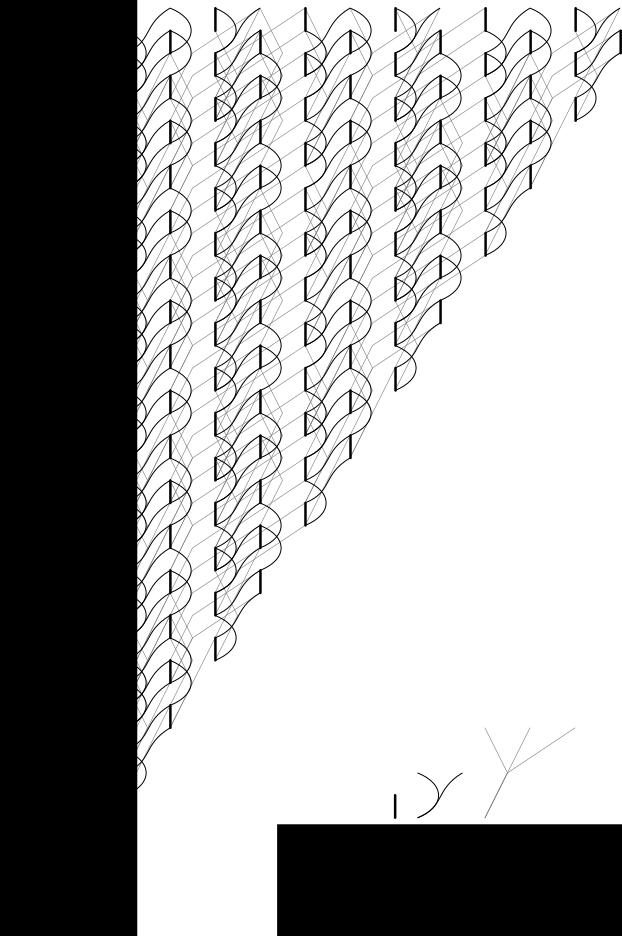
\includegraphics[width=0.9\textwidth]{pics/L2-paper.pdf}
  \caption{The structure of $\L(2)$ as an $\A(2)$-module.  Each point is an element of the Adem basis for $\L(2)$; for example the bottommost point in the first column is $\Sq^0$, while the bottommost point in the second column is $\Sq^2\Sq^1$.  The lines show the action of $\A(2)$; for instance the light gray lines connect each monomial $\Sq^I$ to the terms of $\Sq^4\Sq^I$.  Shifting the diagram down by 8 rows or right by 4 columns shows the periodic structure.  $L(2)$ consists of all but the first column; $\Lkm$ extends infinitely far to the left.\label{fig:L2}}
\end{figure}

If we consider $L(k)$ as a module over $\A(n)$, we find from the Adem relations that it has a nice periodic structure.  In particular, the left action of $\Sq^{2^i}$ commutes with the operation of decreasing each monomial $\Sq^I$ componentwise by the tuple $(d_1, d_2, \ldots, d_k)$ where $d_j$ is divisible by $2^{i+2-j}$ if $j<i+2$, removing the monomial if it is no longer admissible.  This fact follows trivially from the Adem relations; in particular adding a large power of two to the exponent of the second term does not affect the binomial coefficients.

In many cases, that periodic structure becomes somewhat easier to consider if we include all admissible monomials of length \emph{at most} $k$.
\begin{defn}
  Let $\L(k)=\bigcup_{i\leq k}L(i)$ include all admissible monomials of length \emph{at most} $k$.
\end{defn}

For example, the structure of $\L(2)$ as an $\A(2)$-module is shown in Figure~\ref{fig:L2}; it is periodic modulo $(8, 4)$.

In some cases it is simpler to dispense with the edge cases of the periodic structure entirely, and simply extend $L(k)$ back to negative infinity (or equivalently, to the left in Figure~\ref{fig:L2}).  Formally, we let $\Lkm$ consist of admissible monomials composed of factors $\Sq^i$, where $i$ may be negative.  (Admissible monomials are still defined as those in which each term is at least twice the previous one, so that $\Sq^3\Sq^{-2}$ and $\Sq^3\Sq^{-1}$ are both admissible, but $\Sq^{-3}\Sq^{-1}$ is not.)  The module structure of $\Lkm$ over $\A(k)$ may be defined by extending the periodic structure of $L(k)$ backwards, so that $\Sq^{2^i}\Sq^I$ is defined by adding some sufficiently large admissible tuple $J=(2^{i+1}m_1, 2^im_2, \ldots)$ to $I$ so that it becomes positive, performing the multiplication, and then subtracting the tuple $J$ from the exponent of each term of the result, discarding any terms which are no longer admissible.


\subsection{The Wood \boldmath$Z$ basis}
In addition to the Adem basis, the $Z$ basis described by Wood~\cite{TODO} will be important to our work.  Let
\[ X_n = \Sq^{2^{n+1}-2^n}\Sq^{2^{n+1}-2^{n-1}}\cdots\Sq^{2^{n+1}-1}, \]
and let $Z_n = X_n X_{n-1}\cdots X_0$.  Then Wood showed that $Z_n$ is the top element of $\A(n)$, and furthermore that the following is a basis for $\A(n)$.
\begin{defn}
  The Wood $Z$ basis for $\A(n)$ consists of the set of monomials in Steenrod squares produced by multiplying any subset of the Steenrod squares in $Z_n$ in order.
\end{defn}

The Steenrod Algebra, then, consists of all finite subproducts of the infinite product
\[ \cdots\Sq^8\Sq^{12}\Sq^{14}\Sq^{15}\Sq^4\Sq^6\Sq^7\Sq^2\Sq^3\Sq^1.\]

For example,
\[Z_2 = \Sq^4\Sq^6\Sq^7\Sq^2\Sq^3\Sq^1 = \Sq^17 \Sq^5 \Sq^1\]
is the top class of $\A(2)$.  Furthermore, the following set forms a basis of $\A(2)$:
\begin{gather*}
  \Sq^4\Sq^6\Sq^7\Sq^2\Sq^3\Sq^1 \\
  \Sq^4\Sq^6\Sq^7\Sq^2\Sq^3 \quad \Sq^4\Sq^6\Sq^7\Sq^2\Sq^1 \quad \Sq^4\Sq^6\Sq^7\Sq^3\Sq^1 \\
  \Sq^4\Sq^6\Sq^2\Sq^3\Sq^1 \quad \Sq^4\Sq^7\Sq^2\Sq^3\Sq^1 \quad \Sq^6\Sq^7\Sq^2\Sq^3\Sq^1 \\
  \vdots \\
  \Sq^4 \quad \Sq^6 \quad \Sq^7 \quad \Sq^2 \quad \Sq^3 \quad \Sq^1 \\
  1
\end{gather*}

Note that the $Z$ basis builds larger $\A(n)$ from right to left: in particular, $Z_n = X_n Z_{n-1}$, and therefore each element of the $Z$ basis for $\A(n)$ is formed by multiplying some subproduct of $X_n$ by an element of the $Z$ basis for $\A(n-1)$.  This means that the algebras $\A(n)\mmod\A(n-k)$ have a particularly nice representation in the $Z$-basis.

\begin{prop}
  The set of monomials produced by multiplying any subset of the Steenrod squares in $X_n X_{n-1}\cdots X_{n-k+1}$ in any order forms a set of representatives for a basis for the algebra $\A(n)\mmod\A(n-k)$.  In particular, $X_n X_{n-1} \cdots X_{n-k+1}$ is a representative of its top class.
\end{prop}
\begin{proof}
  Consider some element $z$ of the $Z$ basis for $\A(n)$, which must be a subproduct of $X_n X_{n-1}\cdots X_{n-k+1}Z_{n-k}$.  If it contains any Steenrod squares from $Z_{n-k}$, then it can be written $z = xy$ where $x\in \A(n)$ and $y\in \A(n-k)$.  Then in $\A(n)\mmod \A(n-k) = \A(n) \otimes_{\A(n-1)} \F_2$, $z$ is equal to zero.  Otherwise, it is in the proposed basis.  So since a basis of $\A(n)$ must span $\A(n) \mmod \A(n-k)$, the proposed basis must span.  Furthermore, $\A(n)$ has dimension $2^{2^{n+1}-1}$, and therefore $\A(n)\mmod \A(n-k)$ has dimension $2^{2^{n+1}-2^{n-k+1}}$, so since $X_n X_{n-1} \cdots X_{n-k+1}$ is a product of $2^{n+1}-2^{n-k+1}$ Steenrod squares, there are the right number of subproducts, so they must form a basis.  The element $X_n X_{n-1} \cdots X_{n-k+1}$ is the only element in the right degree to be a representative of the top class, so it must in fact be.
\end{proof}

For example,
\[ \Sq^4\Sq^6\Sq^7\Sq^2\Sq^3 \]
is a representative of the top class of $\A(2)\mmod \A(0)$, and the following set forms a basis of $\A(2)\mmod \A(0)$:
\begin{gather*}
  \Sq^4\Sq^6\Sq^7\Sq^2\Sq^3 \\
  \Sq^4\Sq^6\Sq^7\Sq^2 \quad \Sq^4\Sq^6\Sq^7\Sq^3 \\
  \Sq^4\Sq^6\Sq^2\Sq^3 \quad \Sq^4\Sq^7\Sq^2\Sq^3 \quad \Sq^6\Sq^7\Sq^2\Sq^3 \\
  \vdots \\
  \Sq^4 \quad \Sq^6 \quad \Sq^7 \quad \Sq^2 \quad \Sq^3 \\
  1
\end{gather*}

\section{The Commutation Relation}

We now prove a commutation relation involving the $X_n$ which is interesting in its own right, and will prove useful in the remainder of the paper.

\begin{lem}\label{lem:commutation-relation}
  For any positive integers $m$ and $n$,
  \[X_nX_{n-1}\Sq^{2^{n+1}m} = X_n\Sq^{2^{n+1}m}X_{n-1}.\]
\end{lem}

\begin{proof}
  First, we show the following identities by application of the Adem relations:
  \begin{prop}\label{prop:identity-1}
    For any positive integers $m$ and $n$,
    \[\Sq^{2^n-1}\Sq^{2^{n+1}m}=\Sq^{2^{n+1}m+2^n-1}.\]
  \end{prop}
  \begin{prop}\label{prop:identity-2}
    For any positive integers $k$, $m$, and $n$, with $k\leq n$,
    \[\Sq^{2^n-2^k}\Sq^{2^n-2^{k-1}+2^{n+1}m}=\Sq^{2^n-2^k+2^{n+1}m}\Sq^{2^n-2^{k-1}}+\Sq^{2^{n+1}-2^k}\Sq^{2^{n+1}m-2^{k-1}}.\]
  \end{prop}
  \begin{proof}[Proof of Proposition~\ref{prop:identity-1}]
    The Adem relations give us that
  \begin{equation}\Sq^{2^n-1}\Sq^{2^{n+1}m} = \sum_{j=0}^{2^{n-1}-1}\binom{2^{n+1}m-1-j}{2^n-1-2j}\Sq^{2^{n+1}m+2^n-1-j}\Sq^j.\label{eq:identity-1-adem}\end{equation}
    Recall that in $\F_2$, $\binom{p}{q}$ is $1$ if and only if $p$ has a one in every position of its binary expansion that $q$ has a $1$.  Let $2^n>j>0$ and let $2^{\omega(j)}$ be the largest power of $2$ dividing $j$.  Then the binary expansion of $2^{n+1}m-1-j$ ends in $\omega(j)$ ones preceded by a zero, while that of $2^n-1-2j$ ends in a zero and then $\omega(j)+1$ ones, so the binomial coefficient in the Adem relation is zero.  Then the only term of the Adem relation in~\eqref{eq:identity-1-adem} that is nonzero is that when $j=0$, where $2^{n+1}m-1$ ends with $n+1$ ones, while $2^n-1$ consists of $n$ ones.  The result follows immediately.
  \end{proof}
  \begin{proof}[Proof of Proposition~\ref{prop:identity-2}]
    We expand the first and last terms using the Adem relations, and show that they are identical except for the middle term. For convenience, let $d=2^{n+1}(m+1)-2^k-2^{k-1}$, the degree of the elements.
    \begin{align*}
      \Sq^{2^n-2^k}\Sq^{2^n-2^{k-1}+2^{n+1}m} &= \sum_{j=0}^{2^{n-1}-2^{k-1}} \binom{2^n-2^{k-1}+2^{n+1}m-1-j}{2^n-2^k-2j} \Sq^{d-j}\Sq^j \\
      \Sq^{2^{n+1}-2^k}\Sq^{2^{n+1}m-2^{k-1}} &=\sum_{j=0}^{2^n-2^{k-1}}\binom{2^{n+1}m-2^{k-1}-1-j}{2^{n+1}-2^k-2j}\Sq^{d-j}\Sq^j \\
    \end{align*}
    First, let $0\leq j\leq 2^{n-1}-2^{k-1}$; we will show the two binomial coefficients are equal.  We again consider the binary expansions.  The expansion of $2^n-2^k-2j$ is the same as that of $2^{n+1}-2^k-2j$, except that the leading one has been removed.  The corresponding bits of $2^n-2^{k-1}+2^{n+1}m-1-j$ and $2^{n+1}m-2^{k-1}-1-j$ are also zero and one, respectively, so the two binomial coefficients are the same.

    Now let $2^{n-1}-2^{k-1}<j<2^n-2^{k-1}$; we will show that the latter binomial coefficient
    \[\binom{2^{n+1}m-2^{k-1}-1-j}{2^{n+1}-2^k-2j}\]
    is zero.  Let $2^q$ be the next power of $2$ strictly larger than $2^n-2^{k-1}+j$, so $q\leq n-1$.  Then the $q$th position of the binary expansion will not satisfy the condition to make the binomial coefficient one, so it will be zero.

    Finally, if $j=2^n-2^{k-1}$, the binomial coefficient in the second formula has a zero on the bottom, thus is one, so we get $\Sq^{2^n-2^k+2^{n+1}m}\Sq^{2^n-2^{k-1}}$, the middle term of the claimed identity, as the only leftover term, and the identity holds.
  \end{proof}

  Then in particular, by repeated application of the above identities, we may write
  \begin{align*}
    X_{n-1}\Sq^{2^{n+1}m} &= \Sq^{2^n-2^{n-1}}\Sq^{2^n-2^{n-2}}\cdots\Sq^{2^n-2}\Sq^{2^{n+1}m+2^n-1} \\
      &= \Sq^{2^n-2^{n-1}}\cdots\Sq^{2^n-4}\Sq^{2^{n+1}m+2^n-2}\Sq^{2^n-1} \\
      &\quad + \Sq^{2^n-2^{n-1}}\cdots\Sq^{2^n-4}\Sq^{2^{n+1}-2}\Sq^{2^{n+1}m-1}\\
      &\ \;\vdots \\
      &=\Sq^{2^{n+1}m}X_{n-1}\\
      &\quad + \Sq^{2^n-2^{n-1}}\cdots\Sq^{2^n-4}\Sq^{2^{n+1}-2}\Sq^{2^{n+1}m-1}\\
      &\quad + \cdots + \Sq^{2^n}\Sq^{2^{n+1}m-2^{n-1}}\Sq^{2^n-2^{n-2}}\cdots\Sq^{2^n-1}.
  \end{align*}
  Now all of the extra terms are products of (from left to right) an element of $\A(n-1)$, then an element of the form $\Sq^{2^{n+1}-2^k}$ for $k<n+1$, then some element of $\A$.  In particular, they are zero in $\A(n-1)\otimes_{\A(n)}\A$.  Then since $X_n$ is the top class of $\A(n)\otimes_{\A(n-1)}\F_2$, thus annihilates any element of $\A(n)$ that is not in $\A(n-1)$, $1\otimes x\mapsto X_nx$ is well-defined as a map from $\A(n-1)\otimes_{\A(n)}\A$ to $\A$, so the two sides are the same when multiplied by $X_n$:
  \[X_nX_{n-1}\Sq^{2^{n+1}m} = X_n\Sq^{2^{n+1}m}X_{n-1}.\]

\end{proof}

\section{Representatives for \boldmath$\A(n)\mmod\A(n-k)$}


\begin{prop}\label{prop:set-of-reps}
  % There is a set of representatives for a basis of $\A(n)\mmod\A(n-k)$ (in the sense of the above note), all of which lie in $\L(k)$.
  Any element $t$ of $\A(n)$ may be written as $x + yz$ where $x\in \L(k)$, $y\in \A$, and $z\in\A(n-k)\setminus \F_2$ for any $k\geq 0$.  Equivalently, $\A(n)\subset \L(k) + \A(\Sq^i)_{i\leq k}$, where we take $\A(\Sq^i)_{i\leq k}$ to be the left ideal of $\A$ generated by $\{\Sq^i\}_{i\leq k}$, for any $k\geq 0$.
\end{prop}

Proposition~\ref{prop:set-of-reps} essentially says that there exists a set of representatives for a basis of $\A(n)\mmod\A(n-k)$, all of which lie in $\L(k)$.

\begin{proof}
  It suffices to prove the proposition on some basis for $\A(n)$.  Recall that in Wood's Z-basis of the Steenrod algebra, a basis for $\A(n)$ consists of all strings of squares selected from~\eqref{eq:woodz} and multiplied in the given order:
  \begin{equation} \label{eq:woodz}
    \Sq^{2^{n+1}-2^n}\Sq^{2^{n+1}-2^{n-1}}\cdots\Sq^{2^{n+1}-1} \Sq^{2^n-2^{n-1}}\cdots\Sq^{2^n-1}\cdots\Sq^2\Sq^3\Sq^1
  \end{equation}

  We induct on the number of squares selected.  The empty product is $1$, which is in $\L(k)$, so we are done.  So now suppose the proposition holds on all elements of the Wood Z-basis of length at most $l-1$, and let $t$ be an element of length $l$.  Then, for some $m=2^j-2^i$, $i<j\leq n+1$, we may write $t=\Sq^m\left(x+yz\right)$ where $x$, $y$, and $z$ are as in the statement of the proposition.

  Now $\Sq^myz$ is clearly of the prescribed form, since $\Sq^my$ is in $\A$.  If $x\in\L(k-1)$, then $\Sq^m x\in \L(k)$ (since application of the Adem relations cannot increase the length of a monomial), so we may suppose $x\in L(k)$.

  Write $x$ in admissible form as $\Sq^{i_1}\Sq^{i_2}\cdots\Sq^{i_k}$.  If $\Sq^m\Sq^{i_1}\Sq^{i_2}\cdots\Sq^{i_k}$ is already in admissible form, then we have that $2^ki_k\leq 2^{k-1}i_{k-1}\leq\cdots\leq2i_1\leq m<2^{n+1}$, so in particular, $i_k<2^{n-k+1}$, so $i_k\in\A(\Sq^i)_{i\leq k}$, so in fact the entire product $\Sq^mx$ is in $\A(\Sq^i)_{i\leq k}$.  Then we may apply the Adem relations at least once, to get
  \[\Sq^m\Sq^{i_1}\Sq^{i_2}\cdots\Sq^{i_k} = a_0\Sq^{m+i_1}\Sq^{i_2}\cdots\Sq^{i_k} + \sum_{1\leq j\leq \frac{m}2}a_j\Sq^{m+i_1-j}\Sq^j\Sq^{i_2}\cdots\Sq^{i_k};\]
  the first term we know is in $L(k)$.  For each of the remaining terms, if we may repeat the same process, ignoring the first factor; either the product is in $\A(\Sq^i)_{i\leq k}$, or it may be further reduced by the Adem relations.  Finally, if we apply the Adem relations $k$ times, the rightmost factor must be $\Sq^i$ for $i\leq \frac{m}{2^k}<2^{n-k+1}$, so similarly the product lies in the ideal $\A(\Sq^i)_{i\leq k}$.  Then $\Sq^mx$ may be written in the desired form, so we are done.
\end{proof}

\section{Linear Independence}

\begin{lem}\label{lem:li-vs}
  %TODO: is the claim here really that they are LI in the vector space over $\F2$?
  Taken as elements of $\Lkm$ as a vector space over $\F_2$, the set
  \[\{X_nX_{n-1}\cdots X_{n-k+1}\Sq^I\mid I=(2^{n+1}m_1,2^nm_2,\ldots,2^{n-k+2}m_k), m_1\geq\cdots\geq m_k\}\]
  is linearly independent.
\end{lem}
\begin{proof}
  Note that by the commutation relation we have shown, the element $s=X_nX_{n-1}\cdots X_{n-k+1}\Sq^I$ may be rewritten as
  \[X_n\Sq^{2^{n+1}m_1}X_{n-1}\Sq^{2^nm_2}\cdots X_{n-k+1}\Sq^{2^{n-k+2}m_k}.\]
  Let $M_{k,n}$ be the subspace of $\A$ which is spanned by monomials of the form $yz$ where $y\in L(k)$ and $z\in \A(n)$ with the degree of $z$ at least $1$.  If $b\in \A$, we will write $b+M_{k,n}$ for the subset of $\A$ consisting of elements of the form $b+m$ for $m\in M_{k,n}$.

  \begin{prop}\label{prop:m-thing}
    The element
    \[X_n\Sq^{2^{n+1}m_n}X_{n-1}\Sq^{2^nm_{n-1}}\cdots X_{n-k+1}\Sq^{2^{n-k+2}m_{n-k+1}}\]
    is in
    \[\Sq^{2^{n+1}(m_n+n)+1}\Sq^{2^n(m_{n-1}+n-1)+1}\cdots\Sq^{2^{n-k+2}(m_{n-k+1}+n-k+1)+1} + M_{k,n-k}.\]
  \end{prop}
  \begin{proof}

    %TODO: fix gap here: why isn't $X_n$ just in $M_{1, n-1}$ (may just need to show this out)?
  We proceed by induction on $k$ for fixed $n$.  If $k=1$, we know that $X_n\in M_{1,n-1}+\Sq^{n2^{n+1}+1}$, since the latter term is the only element of $L(1)$ in the right dimension.  Then since, as an $\A(n)$-module, $L(1)$ is periodic in degrees modulo $2^{n+1}$, $X_n\Sq^{2^{n+1}m}\in M_{1,n-1}+\Sq^{2^{n+1}(n+m)+1}$.

  Now suppose the proposition holds for some $k$; we will show it for $k+1$.  Let 
  \begin{align*}
  t&=X_n\Sq^{2^{n+1}m_n}X_{n-1}\Sq^{2^nm_{n-1}}\cdots X_{n-k+1}\Sq^{2^{n-k+2}m_{n-k+1}} \\
  t'&=X_{n-k}\Sq^{2^{n-k+1}m_{n-k}} \\
  b&=\Sq^{2^{n+1}(m_n+n)+1}\Sq^{2^n(m_{n-1}+n-1)+1}\cdots\Sq^{2^{n-k+2}(m_{n-k+1}+n-k+1)+1} \\
  b'&=\Sq^{2^{n-k+1}(m_{n-k}+n-k)+1}.
  \end{align*}
  Then by inductive hypothesis we know that $t\in b+M_{k,n-k}$ and by the base case we know that $t'\in b'+M_{1,n-k-1}$; we wish to show that $tt'\in bb'+M_{k+1,n-k-1}$.  To do this, it suffices to show that $bM_{1,n-k-1}$ and $M_{k,n-k}t'$ are contained in $M_{k+1,n-k-1}$; for simplicity we will show that this is true of the spanning sets we have constructed.
  
  %TODO: check this more carefully.
  First, let $y\in L(1)$, $z\in \A(n-k-1)$ with $z$ not in degree $0$, so that $yz\in M_{1,n-k-1}$.  Then by looking at degrees, $by$ is already in admissible form, so it is in $L(k+1)$, so $byz\in M_{k+1,n-k-1}$ as desired.  Since elements of the form $yz$ span $M_{1,n-k-1}$, we get that $bM_{1,n-k-1}\subset M_{k+1,n-k-1}$.

  Second, let $y\in L(k)$, $z\in \A(n-k)$ with $z$ not in degree $0$, so that $yz\in M_{k,n-k}$.  If $z\not\in\A(n-k-1)$, then $zX_{n-k}$ and thus $yzt'$ must be zero in $\A(n-k)$.  Then we may assume $z\in\A(n-k-1)$; we will show that both $yzb'$ and $yzM_{1,n-k-1}$ are contained in $M_{k+1,n-k-1}$.  Now if we write $zb'$ in admissible form, multiplying by $y$ will give an element already in admissible form by looking at degrees, so we need only show that $zb'\in M_{1,n-k-1}$.  If we multiply out using the Adem relations, this is clearly true, modulo showing that $zb'$ contains no terms of length $1$.  This is easy to show; by the Milnor basis, $z$ cannot end in a Steenrod square with degree a multiple of $2^{n-k}$, but $b'$ is a Steenrod square in a degree which is $1$ modulo $2^{n-k}$, so on multiplying the two, the length $1$ term must vanish, as desired.

  %maybe we can merge the following with the previous argument somehow?
  Finally, then, we must show that $yzM_{1,n-k-1}\subset M_{k+1,n-k-1}$; let $y'\in L(1)$ and $z'\in\A(n-k-1)$, so we must show that $yzy'z'\in M_{k+1,n-k-1}$.  Again looking at the Adem relations, we may write $zy'$ in the form $y''z''$ where $y''\in L(1)$ and $z''\in\A(n-k-1)$.  Then $z''z'\in \A(n-k-1)$ and is not in degree zero, and $yy''\in L(k+1)$, so $yy''z''z'\in M_{k+1,n-k-1}$.

  Then the induction is complete; all terms of $tt'-bb'$ are in $M_{k+1,n-k-1}$ as desired.
  \end{proof}

  %TODO: show somewhere that the shortest terms are in fact the shortest, i.e., that all terms of $M_{k, n-k}$ are of length at least $k+1$.
  %TODO: make this argument clearer
  Then since the elements in question may be written in the given form, their shortest terms are unique and distinct, so the terms are linearly independent.
\end{proof}

\section{Filtrations of \boldmath$L(k)$}

\subsection{The General Case}

%TODO: I think we can't use the word basis here, we have to talk about filtrations, or "bases".
Lemma~\ref{lem:li-vs} suggests that the set
\[ B_{n,k} = \{Sq^I \mid I = (2^{n+1}m_1, 2^n m_2, \ldots, 2^{n-k+2}m_k), m_1 \geq \cdots \geq m_k \} \]
may be a basis for $\Lkm$ as an $\A(n)\mmod\A(n-k)$-module, through the following theorem.

\begin{thm}\label{thm:li-module}
  The set $B_{n,k}$ is linearly independent as elements of $\Lkm$ considered as an $\A(n)\mmod\A(n-k)$-module.
\end{thm}

\begin{proof}
  Suppose it were not: suppose that there were some relation $\sum_i x_i b_i = 0$, with $x_i\in\A(n)\mmod\A(n-k)$ and $b_i\in B_{n,k}$.  Let $z$ be the top class of $\A(n)\mmod\A(n-k)$.  We now have two cases.

  %TODO: check that hopf algebra is the right criterion here, and that it's true
  First, consider the case where not all $b_i$ are in the same degree; let $b_j$ be one of the ones in the highest possible degree.  Since $\A(n)\mmod\A(n-k)$ is a Hopf algebra, there exists some $y_j$ in $\A(n)\mmod\A(n-k)$ such that $y_j x_j = z$.  Then for any $b_{j'}$ in a lower degree than $b_j$, the corresponding $x_{j'}$ will be in a higher degree than $x_j$.  Then $y_j x_j = 0$, so multiplying the entire relation by $y_j$ leaves a new relation amongst only the $b_i$ in the highest possible degree.

  So now we consider the case where all $b_i$ are in the same degree.  As before, let $y$ be such that $y x_1 = z$.  Then in the relation $\sum_i y x_i b_i = 0$, the first coefficient is $z$, and all of the later ones are either $z$ or zero.  But each $z b_i$ is an element of the linearly independent set from Lemma~\ref{lem:li-vs}, so there can be no relation among them.  Then we have a contradiction: there is no relation among the $b_i$ over $\A(n)\mmod\A(n-k)$, so the set $B_{n,k}$ is linearly independent.
\end{proof}

Given this, it remains only to show that in some sense the basis $B_{n,k}$ has the right size.  Unfortunately, this is more difficult than it sounds.  If we take the full basis $B_{n,k}$ over $\Lkm$, the vector space of elements in each degree is infinite-dimensional, so the argument cannot proceed.  If we consider only the intersection of $B_{n,k}$ with $\L(k)$, this difficulty is removed, but another one presents itself: some classes are not spanned by the $B_{n,k}$.  While this issue is irrelevant to the desired final result, in that the periodic structure is still entirely encapsulated, with the exception of some initial conditions, a dimension-counting argument would require a careful accounting of these initial exceptions, which we found intractible in the general case.

Thus we were unable to show the desired result in the general case.  We do believe that a proof could proceed along these lines, we have just been unable to complete the dimension-counting portion of the argument, and hope that future research will yield fruits in the area.

\subsection{The case of small \boldmath$n$ and \boldmath$k$}

%TODO: discussion of small cases

%TODO: future work

\end{document}
